\documentclass[12pt]{report}
\usepackage{makeidx}
\usepackage{graphicx}
\usepackage{xcolor}
\usepackage{listings}
\usepackage{float}
\usepackage{minted}
\usepackage[left=2cm,right=2cm,top=2cm,bottom=5cm]{geometry}
\usepackage{soul}
\usepackage{array}
\def\mystrut(#1,#2){\vrule height #1 depth #2 width 0pt}
\newcolumntype{C}[1]{%
   >{\mystrut(3ex,2ex)\centering}%
   p{#1}%
   <{}}
\textwidth 6in
\textheight 9in
\topmargin 0in
\headsep 0in
\oddsidemargin 0.5cm
\evensidemargin -0.5cm

\lstset{basicstyle=\ttfamily,
  showstringspaces=false,
  commentstyle=\color{red},
  keywordstyle=\color{blue}
}

\title{Skyscrapers Puzzle with\\
Altera FPGA DE1}

\date{\vspace{-5ex}}

\begin{document}
\author{Students: Andrea Giardini - Francesco Venturoli}
\maketitle

\chapter*{Aim of the project}

The project aim is to write a software to run the Skyscrapers puzzle on
a Altera DE1 board \cite{AlteraDE1Board}, allowing users to interact with
it using a keyboard. The final result will be an interactive logic game,
where the user can input digits in the board or ask a suggestion for the
next step. The game needs to recognize when the puzzle is completed and if
the solution provided is correct and respects all the constraints.

\begin{figure}[H]
  \centering
  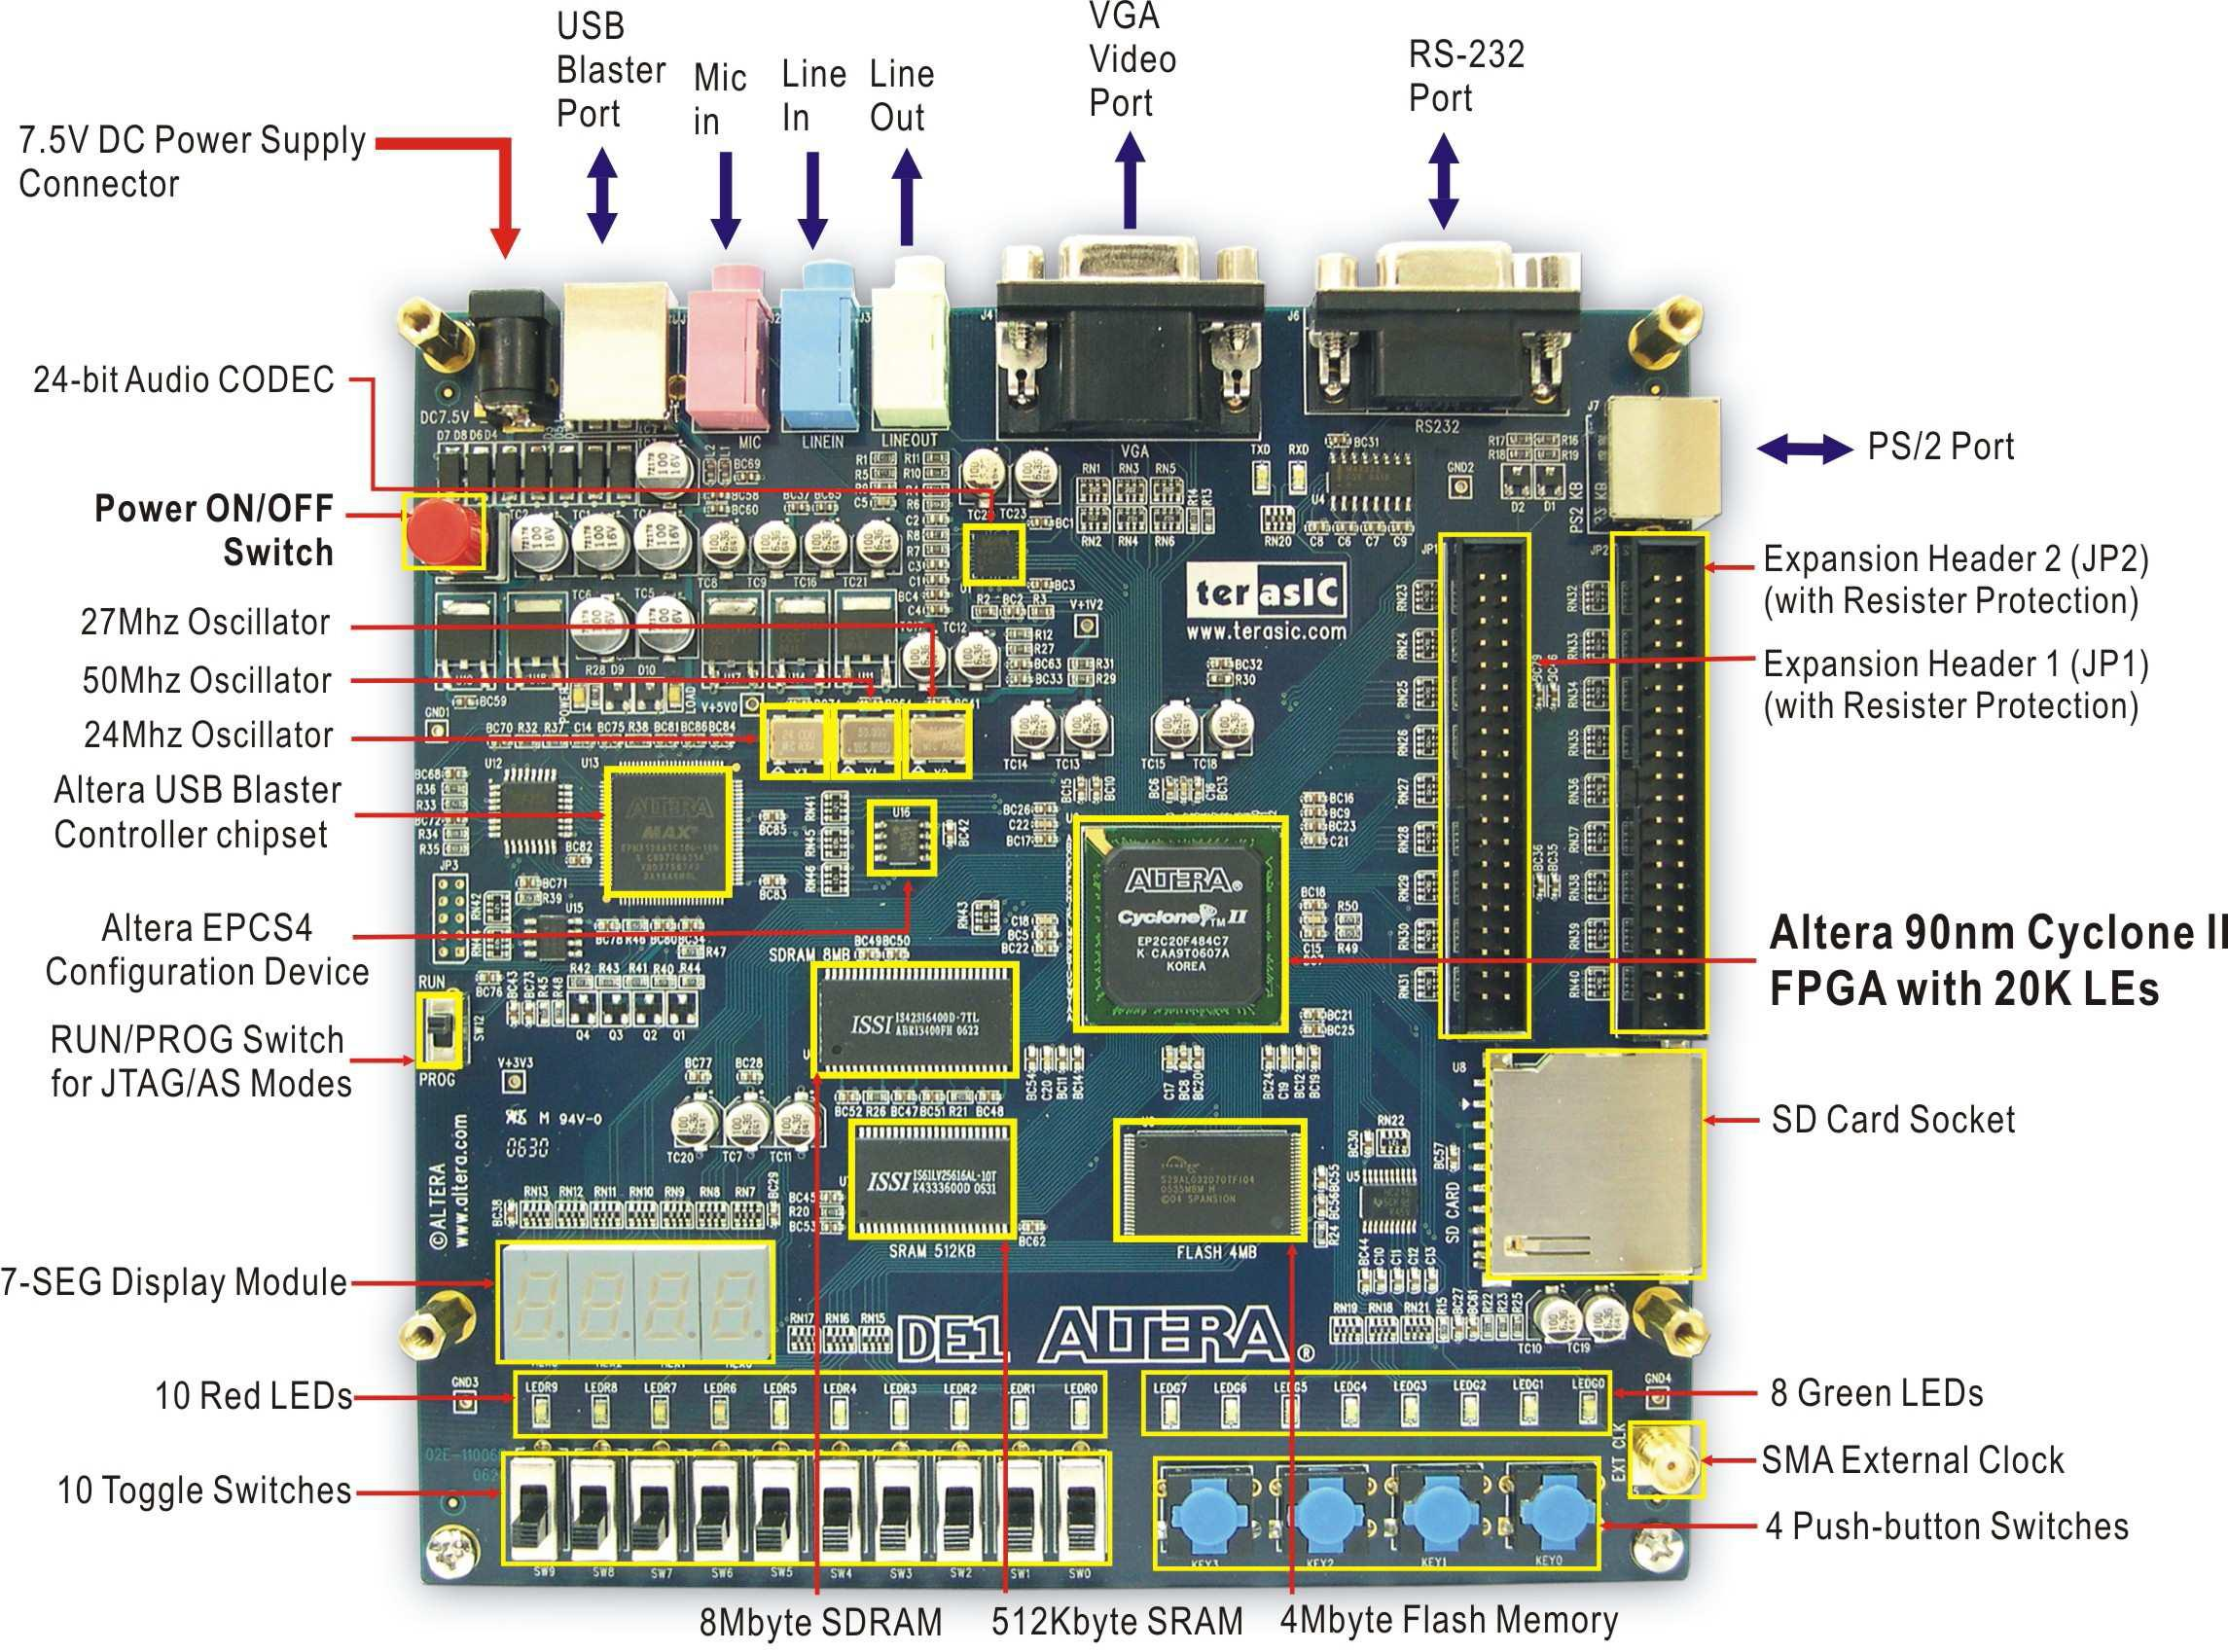
\includegraphics[keepaspectratio,width=0.8\textwidth]{images/Altera_DE1_Board.jpg}
  \caption{Altera DE1 FPGA Board}
\end{figure}

In the proposed game the user needs to be able to move in the game using
the cursors of the keyboard. Entering numbers in the matrix, always using
the keyboard, the user tries to complete the puzzle filling all the blank
spaces with a numeric value. If the user is not able to complete the game
it can solve the board automatically using the algorithms implemented in
the board. Once the puzzle is solved, the board should recognize the
solution and display the winning logo to the user.

\chapter*{Introduction to the puzzle}

Each puzzle consists of an NxN grid with some clues along its sides. The
goal is to place a skyscraper in each square, with a height between one
and N, so that no two skyscrapers in a row or column have the same number
of floors. In addition, the number of visible skyscrapers, as viewed from
the direction of each clue, is equal to the value of the clue. Note that
higher skyscrapers block the view of lower skyscrapers located behind
them.

\begin{figure}[H]
  \centering
  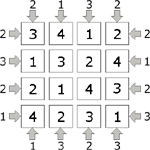
\includegraphics[keepaspectratio]{images/skyscrapers_small_solved.jpg}
  \caption{Solved 4x4 Skyscrapers puzzle}
\end{figure}

There are a number of intuitions that can be addressed immediately,
filling some of the empty spaces with values, others spaces instead need
a combination of more constraints to identify the correct value. The game
can be extended with a bigger matrix or to include parks ( empty spaces, so
buildings with zero height in the matrix ). In our case we decided to
solve the classic version of the puzzle, a 4x4 matrix with no parks.

\newpage

\section*{Control Unit}

The control unit is used in this project to get the inputs from the user
and interpret them. Following that, the interpreted signal is sent to
the Datapath or the View depending on which kind of change we want to
address.

As we specified previously, our intention is to let the user use
a keyboard to play the game. In order to do this we have to read the
serial PS2 line and map the received data with the scan codes of the
keys that we wanted to interpret.

To simplify the problem and keep the Control Unit as clean as possible
we added a new class called \textit{Skyscrapers\_Puzzle\_Keyboard} which is
responsible exclusively to read the data from the keyboard and map it to
scan codes. Using this class we can leave all the logic of translating
the signals to actions to the Control Unit, as it is supposed to be.

The Control Unit has the following signals:

\begin{center}
\begin{minipage}{0.5\textwidth}
\begin{minted}{vhdl}
  CLOCK        : in std_logic;
  keyboardData : in std_logic_vector (7 downto 0);
  RESET_N      : in std_logic;
  TIME_10MS    : in std_logic;

  CURSOR_POS   : in CURSOR_POS_TYPE;

  -- Connections with Data-Path
  MOVE_RIGHT   : out std_logic;
  MOVE_LEFT    : out std_logic;
  MOVE_DOWN    : out std_logic;
  MOVE_UP      : out std_logic;
  NUMBER       : out std_logic_vector (3 downto 0);
  SOLVE        : out std_logic;
  CLEAN        : out std_logic;
\end{minted}
%\caption{Input and Output signals for Control Unit}
\end{minipage}
\end{center}

The Control Unit reads the serial line \textit{KEYBOARDDATA} and
interprets the scan codes received in actions, that are then sent to the
Datapath. In order not to consider a single press as multiple (since the
clock data is fast) we are scanning the line periodically and not
constantly.

\newpage

\section*{Datapath}

The Datapath takes care of the logic of the game, it maintains in memory
the numbers that the user added to the matrix. The user is able to add new
numbers to the matrix from the keyboard and all its changes are registered
inside the Datapath. Moreover, the Datapath contains all the logic to
solve the puzzle.

\begin{center}
\begin{minipage}{0.5\textwidth}
\begin{minted}{vhdl}
  CLOCK       : in std_logic;
  RESET_N     : in std_logic;
  MOVE_RIGHT  : in std_logic;
  MOVE_LEFT   : in std_logic;
  MOVE_DOWN   : in std_logic;
  MOVE_UP     : in std_logic;
  SOLVE       : in std_logic;
  CLEAN       : in std_logic;

  KEYS        : in std_logic_vector (3 downto 0);

  MATRIX      : out MATRIX_TYPE;
  CONSTRAINTS : out CONSTRAINTS_TYPE;
  SOLUTIONS   : out SOLUTIONS_TYPE;
  CURSOR_POS  : out CURSOR_POS_TYPE;
  WINNER      : out std_logic
\end{minted}
%\caption{Input and Output signals for Datapath}
\end{minipage}
\end{center}

The Datapath is the main component of the project since it stores the
matrix with the values, handles the inputs received from the Controller
and contains the algorithm to solve the puzzle.

Every cell in the schema, contains initially all the possible values that
can be assigned to that cell. Using the constraints and the input of the
users the datapath removes possible solutions from the surrounding cells.
Whenever a cell has only one possible solution that value is assigned to
it and displayed on screen.

\newpage

\section*{View}

The View is responsible for drawing on screen the elements of the Datapath
and represent them in the best way for the user. In our case the game is
quite simple to represent on screen but there were some challenges to be
solved, in particular with the drawing of numbers.

\begin{center}
\begin{minipage}{0.5\textwidth}
\begin{minted}{vhdl}
  CLOCK        : in std_logic;
  RESET_N      : in std_logic;

  MATRIX       : in MATRIX_TYPE;
  SOLUTIONS    : in SOLUTIONS_TYPE;
  CONSTRAINTS  : in CONSTRAINTS_TYPE;
  CURSOR_POS   : in CURSOR_POS_TYPE;

  REDRAW       : in  std_logic;

  FB_READY     : in  std_logic;
  FB_CLEAR     : out std_logic;
  FB_DRAW_RECT : out std_logic;
  FB_DRAW_LINE : out std_logic;
  FB_FILL_RECT : out std_logic;
  FB_FLIP      : out std_logic;
  FB_COLOR     : out color_type;
  FB_X0        : out xy_coord_type;
  FB_Y0        : out xy_coord_type;
  FB_X1        : out xy_coord_type;
  FB_Y1        : out xy_coord_type;
  HEX0         : out std_logic_vector (6 downto 0);
  HEX1         : out std_logic_vector (6 downto 0);
  HEX2         : out std_logic_vector (6 downto 0);
  HEX3         : out std_logic_vector (6 downto 0)
\end{minted}
%\caption{Input and Output signals for View}
\end{minipage}
\end{center}

As we can see from the signals, we used the FrameBuffer technology to draw
the frames of the game before printing them on the screen. The FrameBuffer
is a portion of memory containing a Bitmap that is used to refresh a video
display from a memory buffer containing a complete frame of data.
Basically what happens is that we draw the whole frame to be displayed in
memory before actually displaying it on video. Once the frame is ready to
be displayed and all the drawing operations are completed we refresh the
screen putting on it the new frame that we just drawn in memory.

\newpage

The View is organized in different macro states:

\begin{minted}{vhdl}
type state_type is (IDLE, WAIT_FOR_READY, DRAWING);
\end{minted}

In particular we will analyse the DRAWING state, which is made of a set of
sub-states:

\begin{minted}{vhdl}
type substate_type is (CLEAR_SCENE, DRAW_BOARD_OUTLINE, DRAW_BOARD_BLOCKS,
     DRAW_BOARD_CONSTRAINTS, DRAW_BOARD_NUMBERS, FLIP_FRAMEBUFFER);
\end{minted}

Every state draws a different object:

\begin{itemize}
  \item CLEAR\_SCENE

  Cleans the frame in memory, filling it with a black square which will be
  the background of our game.

  \item DRAW\_BOARD\_OUTLINE

  Draws the outline of our game board, just the perimetral square.

  \item DRAW\_BOARD\_BLOCKS

  Draws the blocks inside our game board and the position of the cursor.

  \item DRAW\_BOARD\_CONSTRAINTS

  Draws the constraints around our game board.

  \item DRAW\_BOARD\_NUMBERS

  Places the numbers that have been inserted inside the board.

  \item FLIP\_FRAMEBUFFER

  This state is reached when the drawing has been completed and we are
  ready to display it on the screen.
\end{itemize}

The most difficult part was drawing the numbers on screen since the
FrameBuffer library was not giving us any possibility of drawing custom
images but only squares. To draw the numbers we had to define every digit
as an array of colors, representing pixel by pixel the color that has to
be placed. Following that we had to draw a square of 1x1 pixel for each
pixel of the number's sprite.

\chapter*{Solving algorithm}

In order to solve the puzzle we had to implement in VHDL multiple methods
to insert solutions on the board based on the constraints of the game. In
the following section we will analyse the rules that we are applying to
solve the problem and how they help us to remove possible solutions from
the board.

Starting with the structure, we represented the board as
a three-dimensional matrix. This matrix has dimension 4 (length)
x 4 (height) x 4 (possible solutions). We must consider that, when
a number is inserted, that solution can be removed from the corresponding
row and column, since we cannot have the same number twice on the same
column or row.

During the analysis phase we determined that the most convenient technique
to set the correct value for a cell is to remove, from the set of possible
solutions, all the values that are incorrect. In this way, when a cell has
only a possible value, we set that value.

Rules:

\begin{itemize}

    \item \ul{The constraint is \textbf{one} when the first element
    is \textbf{four}}

    Since only a single skyscraper is visible from that side, it means
    that it must be the tallest one. In this case the number \textit{four}
    is added to the matrix in first position.

\begin{center}
  1
  \begin{tabular}{| C{0.5cm} | C{0.5cm} | C{0.5cm} | C{0.5cm} |}
    \hline
    4 &  &  &  \tabularnewline \hline
  \end{tabular}
\end{center}

    \item \ul{The constraint is \textbf{two} when the second
    element cannot be \textbf{three}}

    If the constraint is two and the second element is three it is not
    possible to match the requirements. In fact, in the best case, it will
    always be possible to see the skyscrapers three, four and the one
    occupying the first place.

    The table below shows an example of this rule, which makes evident
    than the \textit{three} \ul{cannot} be assigned to the second
    position:

\begin{center}
  2
  \begin{tabular}{| C{0.5cm} | C{0.5cm} | C{0.5cm} | C{0.5cm} |}
    \hline
    & 3 &  & 4 \tabularnewline \hline
  \end{tabular}
\end{center}

    \item \ul{The constraint is \textbf{four} when row/column is
    ordered}

    Since the user is able to see all the skyscrapers it means that they
    must be ordered on the line based on their height.

\begin{center}
  4
  \begin{tabular}{| C{0.5cm} | C{0.5cm} | C{0.5cm} | C{0.5cm} |}
    \hline
   1 & 2 & 3 & 4 \tabularnewline \hline
  \end{tabular}
\end{center}

    \item \ul{The opposite constraints are \textbf{two} and
    \textbf{three} when the \textbf{four} is in the second position
    starting from the lowest constraint}

    The skyscraper with height four is always seen from both sides since
    it is the tallest one. This rule can be summarized with: if the
    constrain it X then 4 is in the X position or later.

    If the constraints are two and three, we can define precisely the
    position of the tallest skyscraper, as we can see from the tables
    below.

\begin{center}
  2
  \begin{tabular}{| C{0.5cm} | C{0.5cm} | C{0.5cm} | C{0.5cm} |}
    \hline
    & 4 &  &  \tabularnewline \hline
  \end{tabular}
  3
\end{center}

\begin{center}
  3
  \begin{tabular}{| C{0.5cm} | C{0.5cm} | C{0.5cm} | C{0.5cm} |}
    \hline
    &  & 4 &  \tabularnewline \hline
  \end{tabular}
  2
\end{center}

    It is possible to specify a more general rule, from which we deducted
    this one, that says: the constraint is X when \textbf{four} is in
    position X or more. This means that if the constraint is \textbf{two}
    then the number \textbf{four} can be in the second, third or fourth
    position, but not first. If the constraint is \textbf{three} then the
    number \textbf{four} can be in the third or in the fourth position.
    The combination of these constraints on the opposite side of the same
    row gives us a precise position for the number \textbf{four} in the
    line.

\end{itemize}

The rules that we described previously can help us to reduce the number of
possible solutions in one cell. Unfortunately, just using those rules, our
game is still not able to resolve some obvious cases, like for example:

\begin{center}
  3
  \begin{tabular}{| C{0.5cm} | C{0.5cm} | C{0.5cm} | C{0.5cm} |}
    \hline
    & 2 & 4 &  \tabularnewline \hline
  \end{tabular}
  2
\end{center}

\begin{center}
  3
  \begin{tabular}{| C{0.5cm} | C{0.5cm} | C{0.5cm} | C{0.5cm} |}
    \hline
    &  & 4 & 1 \tabularnewline \hline
  \end{tabular}
  2
\end{center}

In the examples, both empty cells have two possible solutions and, for this
reason no number is assigned to them. We can also notice that, for each
example, there are two possible solution and that only one of them is
correct.

The intuitive rule tries to address this problem, when the number of
possible combinations in a row is two the algorithm tries to verify which
one of them is correct. This rule allowed us to solve more complex
schemas, where the intuition of the user was needed to complete the board.

\chapter*{Conclusion}

The game presented is complete and functional in all its aspects. The
algorithm studied to solve the game introduced a noticeable complexity
from the logic point of view. Due to this we reached the logic limits of
the board: the current project fits on the board just after a heavy
optimization.

\section*{Future developments}

Currently the limits of the board have been reached so the space for
possible developments is quite small. However, with some hard optimization
of the code or with a board with more memory, the following improvements
could be coded:

\begin{itemize}

    \item Generate boards dynamically

\end{itemize}

\renewcommand{\bibname}{References}
\begin{thebibliography}{100}

\bibitem{AlteraDE1Board} http://de1.terasic.com/

\end{thebibliography}

\end{document}
